% Based on LLNCS.DEM the demonstration file of the LaTeX macro package from Springer-Verlag for LNCS version 2.4 for LaTeX2e as of 16. April 2010
%
% Moved LNCS Template's code to a separate file
\input{LNCSTemplate/header.tex}
%
%\usepackage{makeidx}  % allows for indexgeneration
%
\begin{document}
%
\frontmatter          % for the preliminaries
%
\pagestyle{headings}  % switches on printing of running heads
\addtocmark{Hamiltonian Mechanics} % additional mark in the TOC
%
%
%
\mainmatter              % start of the contributions
%
\title{Towards Incentive-based Resource Assignment and Regulation in Clouds for Community Networks}
%
\titlerunning{Resource Regulation in Clouds for Community Networks}  
% abbreviated title (for running head) also used for the TOC unless \toctitle is used
%

\author{ Amin M. Khan \and \"Umit C. B\"uy\"uk\c{s}ahin \and Felix Freitag }
%
\authorrunning{A. M. Khan, \"U. C. B\"uy\"uk\c{s}ahin, and F. Freitag} % abbreviated author list (for running head)
%
%%%% list of authors for the TOC (use if author list has to be modified)
\tocauthor{Amin M. Khan, \"Umit C. B\"uy\"uk\c{s}ahin, and  Felix Freitag}
%
\institute{
    Department of Computer Architecture\\
    Universitat Polit\`ecnica de Catalunya, Barcelona, Spain\\
    \email{ \{mkhan, ubuyuksa, felix\}@ac.upc.edu }\\
}

\maketitle              % typeset the title of the contribution

\begin{abstract}
Community networks are built with off-the-shelf communication equipment aiming to satisfy a community's demand for Internet access and services. These networks are a real world example of a collective that shares ICT resources. But while these community networks successfully achieve the IP connectivity over the shared network infrastructure, the deployment of applications inside of community networks is surprisingly low. Given that community networks are driven by volunteers, we believe that bringing in incentive-based mechanisms for service and application deployments in community networks will help in unlocking its true potential. We investigate in this paper such mechanisms to steer user contributions, in order to provide cloud services from within community networks. From the analysis of the community network's topology, we derive two scenarios of community clouds, the local cloud and the federated cloud. We develop an architecture tailored to community networks which integrates the incentive mechanism we propose. In simulations of large scale community cloud scenarios we study the behaviour of the incentive mechanism in different configurations, where slices of homogeneous virtual machine instances are shared. Our simulation results allow us to understand better how to configure such an incentive mechanism in a future prototype of a real community cloud system, which ultimately should lead to realisation of clouds in community networks.

\keywords{incentive mechanisms, cloud computing, community networks, distributed resource sharing}
\end{abstract}
%

%% *** Introduction

% Section: INTRODUCTION
\section{Introduction}
\label{sec:introduction}

Community networks aim to satisfy a community's demand for Internet access and services using open unlicensed wireless spectrum and off-the-shelf communication equipment. 
Most community networks originated in rural areas which commercial telecommunication operators left behind when focusing the deployment of their infrastructure on urban areas. 
The lack of broadband access brought together different stakeholders of such geographic areas to team up and invest, create and run a community network as an open telecommunication infrastructure based on self-service and self-management by the users~\cite{Elianos2009}.

These community networks are a real world example of a collective that shares information and communication technology (ICT) infrastructure and human resources. 
The ICT resources shared are the bandwidth of the wireless network formed by the networking hardware belonging to multiple owners. 
This bandwidth allows members of the community network obtaining access to the Internet or use services and applications inside of the community network.
The human resources shared are the time and knowledge of the participants, needed to maintain the network and technically organise it for further growth. 

Sharing of network bandwidth has early been identified as essential and is part of the membership rules or peering agreements of many community networks, which regulate the usage and growth of the network. 
The Wireless Commons License (WCL)~\cite{WCL2012} of many community networks states that the network participants that extend the network, e.g. contribute new nodes, will extend the network in the same WCL terms and conditions, allowing traffic of other members to transit on their own network segments. Since this sharing is done by all members, community networks successfully operate as IP networks. 

Today's Internet, however, is more than bandwidth resources. 
Computing and storage resources are shared through Cloud Computing, offering virtual machine instances over infrastructure services, APIs and support services through platform-as-a-service, and Web-based applications to end users through software-as-a-service. 
These services, now common practice in today's Internet, hardly exist in community networks~\cite{Khan2013Clouds}. 
Services offered in community networks still run on machines exclusively dedicated to a single member. 
Community network members, however, do use commercial cloud solutions, for instance for network administration, where sometimes a commercial storage service is used for node data. 
Why have clouds not emerged inside of the community networks?

We argue that community cloud, a cloud infrastructure formed by community-owned computing and communication resources, has many technical and social challenges so that the main drivers of today's contribution to community networks, voluntariness and altruistic behaviour, are not enough to successfully cope with it. 
Our hypothesis is that for community cloud to happen, the  members' technical and human contribution needed for such a cloud, needs to be steered by incentive mechanisms that pay back the users' contribution with a better quality of experience for them.

In this paper, we present an incentive mechanism tailored to community networks.
The main contributions of this paper are the following:
\begin{enumerate}
    \item From the analysis of the key socio-technical characteristics of community networks, we identify two scenarios for community clouds, the local clouds and federated clouds, for which a community cloud management system is proposed.
    \item We design an incentive mechanism that is part of the community cloud architecture and evaluate its behaviour in simulations of community cloud scenarios. 
\end{enumerate}


We elaborate our contributions in the following way: In section~\ref{sec:design} we present our system model and design.
In section~\ref{sec:evaluation}, we evaluate our incentive mechanism in a community cloud scenario.
In section~\ref{sec:related-work} we relate the work of other authors with our results. We discuss open issues in section 5 on future work and in section~\ref{sec:conclusion} we conclude our findings.


%% *** Section: System Model, Architecture and Design
%
%% Section: ARCHITECTURE & DESIGN
%\section{Architecture and Design}
%\label{sec:design}
%
%The option for enabling a community cloud in a community network on which we focus here is to deploy on SNs a cloud management system tailored to community networks. 
%Available popular cloud management platforms, notably
%	OpenStack~\cite{OpenStack} and
%	OpenNebula~\cite{Moreno-Vozmediano2012}
%among others, can principally be applied to provide the basic management of local clouds.
%Such cloud management systems can be tailored for community networks by extending the existing functionality to address the particular conditions of community networks.
%For example, incentive mechanisms inspired by the social nature of community networks can be built 
%into resource regulation component to encourage users to contribute resources~\cite{Khan2014Prototyping, Khan2013TowardsIncentives}. 
%
%
%\subsection{Community Cloud Management System}
%
%
%The architecture for the cloud management platform that we propose for community networks
%consists of multiple layers~\cite{Khan2014Architecture}, 
%with different components at each layer, as shown in Figure~\ref{fig:overview-vmm-hierarchy}.
%
%%% FIGURE
%\begin{figure}[tbp]
%	\centering
%	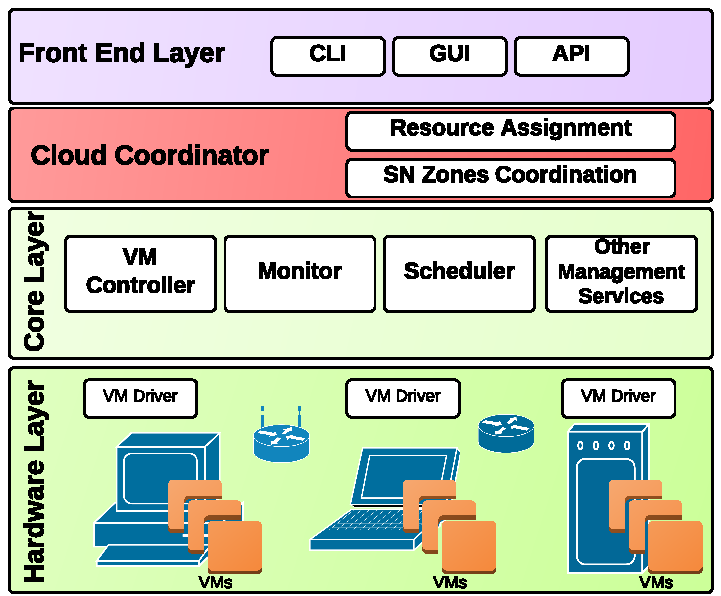
\includegraphics[width=3.5in, keepaspectratio]{vmm-architecture-generic}
%	\caption{Architecture of cloud management system}
%	\label{fig:overview-vmm-hierarchy}
%\end{figure}
%
%\subsubsection{Hardware Layer}
%This consists of the physical infrastructure that is needed to run a cloud system. 
%The hardware in the community networks mostly consists of ONs and SNs and the communication infrastructure, along with any attached computation, storage and other resources.
%
%\subsubsection{Core Layer}
%The core layer consists of components that are responsible for creation, allocation, scheduling, monitoring and management of VMs on the nodes. 
%This can include the following components, some of which are shown in Figure~\ref{fig:overview-vmm-hierarchy}.
%
%\begin{itemize}
%    \item Virtual Machines Controller
%    \item Virtual Machines Scheduler
%    \item Virtual Machines Monitor
%    \item Hosts Manager
%    \item Virtual Network Manager
%    \item Virtual Machines Image Data Store
%\end{itemize}
%
%The functionality of the core layer is already provided by tools like OpenStack and others.
%Community cloud manager can, therefore, make use of these existing tools and extend their functionality to suit the needs of the community network.   
%
%
% %%%%%%%%%%%%%%%%%%%%%%%%%%%%%%%%%%%%%%%%
%\subsubsection{Cloud Coordinator}
%The cloud coordinator is responsible for the federation of the cloud resources which are independently managed by different SNs.
%The cloud coordinator components in different SNs connect among themselves in a decentralised manner to exchange relevant information about managing the available resources.
%Normally applications running at a local community cloud can only consume resources from the ONs directly managed by that particular SN.
%With the cloud coordinator, the infrastructure service can provide a unified view of the resources contributed by multiple local community clouds.
%Figure~\ref{fig:cloud-coordinator-arch} shows the implemented components of the cloud coordinator in the prototype as described below.
%
%\begin{itemize}
%
%    \item{ON Management:} ONs can register with SN to request and to contribute resources.
%
%    \item{Regulation Mechanism:} When pooling resources from multiple zones, the cloud coordinator applies a regulation mechanism that takes into account resource utilisation and contribution by different nodes to perform resource allocation. 
%
%    \item{SN Interconnectivity:} The design of a community cloud manager follows a decentralised approach, so cloud coordinator relies on gossip-based discovery mechanisms to manage overlay network of the SNs in community cloud.
%    The updated list of adjacent SNs is saved in SN-List database.
%
%    \item{SN Resource Sharing:} When requests from ONs cannot be met from locally available resources, SN can request resources from other SNs in the system.
%
%\end {itemize}
%
%%% FIGURE
%\begin{figure}[tbp]
%	\centering
%	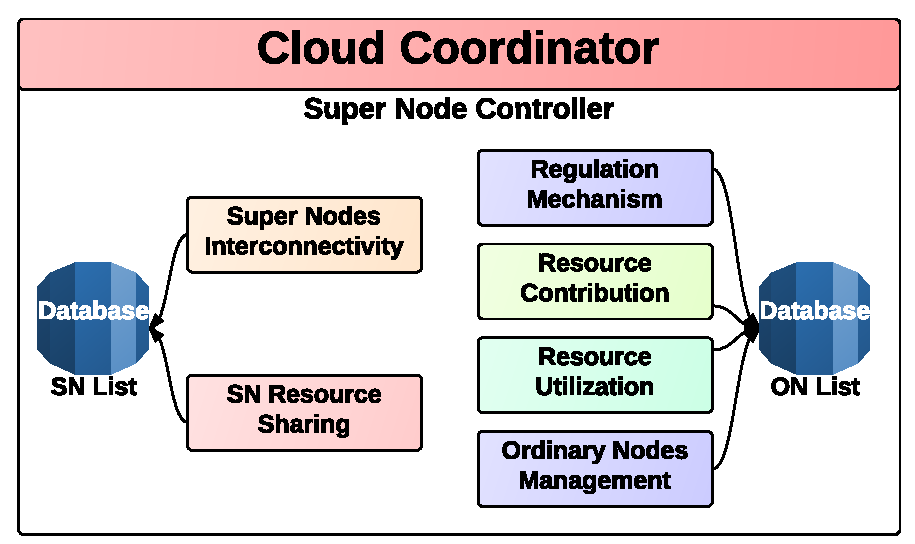
\includegraphics[width=3.5in, keepaspectratio]{vmm-cordinator-arch}
%	\caption{Components of cloud coordinator}
%	\label{fig:cloud-coordinator-arch}
%\end{figure}
%
%
%\subsubsection{Frontend Layer}
%The frontend layer provides the interface to interact with the infrastructure service of the community cloud. 
%This includes modules like command line interface (CLI), graphical user interface (GUI), application programming interface (API), and any other tools that assist with developing cloud application using the infrastructure service.  
%
%
%%%%%%%%%%%%%%%%%%%%%%%%%%%%%%%%%%%%%%%%%
%\subsection{Interaction between Super and Ordinary Nodes}
%
%The overlay network that results from the hierarchical architecture of the community cloud is formed by SNs.
%The difference between SNs and ONs, from the point of view of cloud management, is that SNs support greater functionality for handling VMs. 
%A SN has full installation of the cloud management software and so enables the user to manage VMs executing on ONs.
%In most cases, a SN will be a comparatively stable node, most likely connected to a hub of the wireless mesh network. 
%Each SN is responsible for a set of ONs and manages their metadata in its ON-List database. 
%SNs publish their status and details of local resources to other SNs, e.g. by gossiping, and each SN stores this information in SN-List database.
%ONs, on the other hand, only act as hosts for executing VMs. 
%Most components of cloud management software are not installed on ONs, so the VMs cannot be controlled conveniently from the ONs themselves.
%Each ON registers to a parent SN by providing it with the list of the available resources, and the parent SN is responsible for management of VMs. 
%ONs periodically send a heartbeat message to their parent SN to inform it about their current status.
 

% *** Section: Evaluation/Experiments

% Section: EVALUATION
\section{Performance Evaluation}
\label{sec__dist_auctioneer_evaluation}

We have evaluated the implementations of the allocator for double and standard auctions proposed in \Cref{sec__dist_auctioneer_instances}.
The implementations of all the remaining blocks are as suggested in \Cref{sec__distrib_auctioneer_protocol_implementation}: 
we use the rational consensus algorithm proposed in~\cite{Afek2014} in the implementation of the bid agreement, 
while the input validation and data transfer blocks are implemented as simple broadcasts, 
and the common coin is implemented using the scheme from~\cite{Abraham2013}. 
For these implementations to be $k$-resilient equilibria, we need $m>2k$. 
This is a requirement of the rational consensus algorithm. 

Our goal is to assess the overhead of the distributed protocol, when compared to a purely centralised solution,
in the case the allocation algorithm is not parallelisable, 
and to assess the potential benefits from parallelisation when computationally expensive allocation algorithms are used. 
For that purpose, we measure performance gains for different levels $p$ of parallelism, where $p = \lfloor m/(k+1) \rfloor$ is the maximum level of parallelism for each possible $k$ and $p=1$ represents the sequential execution by a trusted auctioneer.
We consider a fixed number of $m=8$ providers in the auctions,
but we vary the number of providers that execute each protocol.

\subsection{Hardware/Software Setup}

In order to obtain a meaningful evaluation of our approach, we have resorted to a prototype implementation on realistic hardware and software environment and deployed it in an experimental testbed for community networks, namely on nodes of the Guifi.net, one of the largest community networks in the world~\cite{ClommunityTestbed}. 
We were given access to 4 different nodes of the experimental testbed, 2 machines in Barcelona (UPC Campus), and one machine each in Barcelona (Hangar) and in Taradell, Spain.
When doing tests executed by more than 4 providers we have instantiated 
multiple VMs in each nodes, ensuring that each VM is allocated a different CPU. 
The machines are Intel Core i7-3770 3.40GHz CPU with 16 GB RAM and 1 TB hard disk, running Proxmox virtualisation engine. 
Our experiment runs in OpenVZ containers with Debian 7 x86 1 CPU, 2 GB RAM, and 10 GB storage. 
We have implemented the framework in Python, using PyPy for speed reasons, 
and used \O{}MQ~\cite{ZeroMQ} as the messaging library for the communication.

We have set up a single node that acts as a client, and generates input for all the $n$ users.
This client node sends the requests to the $m$ providers, and receives the results back from all of them.
The values for running time presented in the plots capture the time from when the inputs are generated at this client node,
till the time it receives the results from all the experiment instances.
We run the experiments for 100 rounds, and plot the average values in the graphs.

\subsection{Double Auction Deployment}

We have used an experimental set up similar to~\cite{Zheng2014Star}, with some slight modifications suitable to our use case.
In both the experiments, the double and standard auction, 
the bids by the users are uniformly distributed in the range $[0.75, 1.25]$,
and the requested bandwidth resource is uniformly distributed in the range $(0, 1]$.
We vary the capacity of the providers depending upon the overall bandwidth required, and scale it using a random factor in $[0.5, 1.5]$ so as to consider both the cases where providers lack the capacity to satisfy all the requests, and where the providers have excess capacity.
The providers have a unit cost of bandwidth uniformly distributed in the range $(0, 1]$.

%% FIGURE
\begin{figure}[tbp]
	\centering
	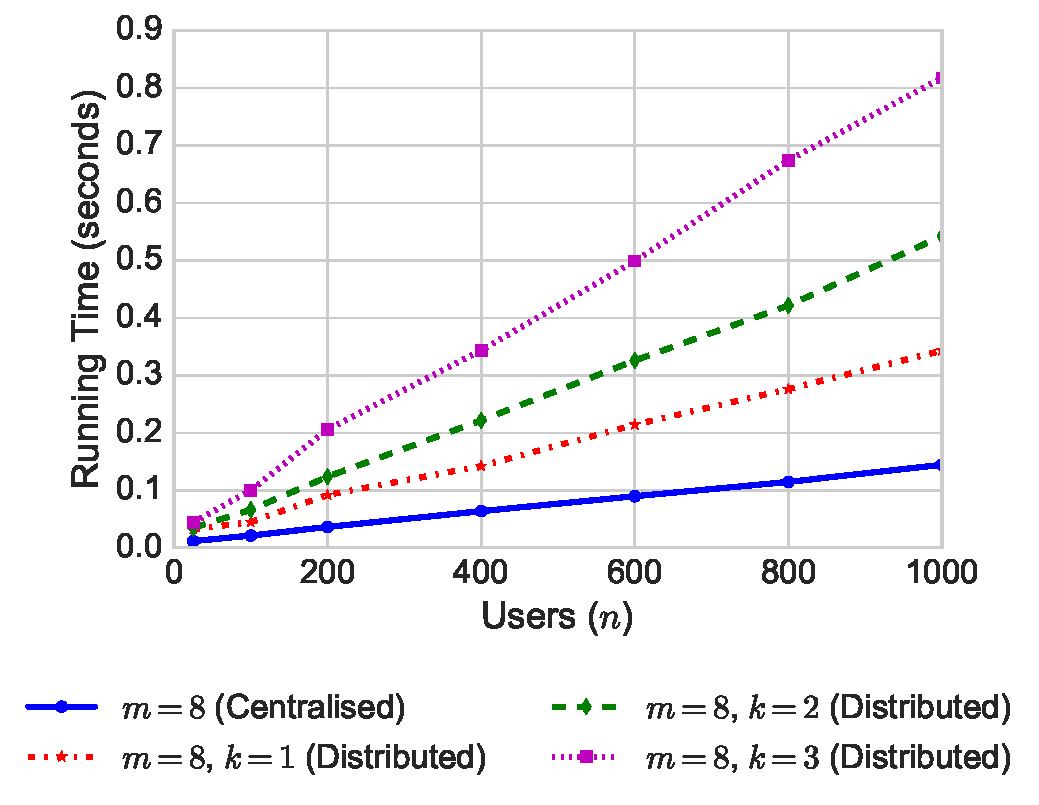
\includegraphics[width=0.65\columnwidth,keepaspectratio]{time-double-auction}
	\caption{Running time for double auction}
	\label{fig:double-auction-time}
\end{figure}

Figure~\ref{fig:double-auction-time} shows the running time for the double auction algorithm (\Cref{sec:instances-double-auction}) 
as a function of the number of users, for up to 1000 users. 
This algorithm has little computational overhead. 
It is not easily parallelisable but, as it can be observed from the figure, this is irrelevant as the distributed version is dominated by the communication time. 
Also, the communication overhead increases as the number of users increases, since more data has to be exchanged between the providers. 
The figure shows the values obtained for the centralised approach and for the distributed implementation using different values of $k$
and corresponding minimum required number of providers out of a total of 8 involved in the execution, namely, $3$ providers when $k=1$, $5$ when $k=2$, and $8$ when $k=3$. 
Even when 8 providers and 1000 users are used, the 
distributed implementation finishes in less than a second which is perfectly 
acceptable because normally these auctions need to run with reasonable intervals between them.

\subsection{Standard Auction Deployment}

We fix the number of providers to $m=8$ and vary the maximum degree of parallelisation 
by taking $p$ to be $1$, $2$, and $4$, corresponding to a centralised execution, $k=3$, and $k=1$, respectively.
Figure~\ref{fig:standard-auction-time} shows the running time for the standard 
auction (\Cref{sec:instances-vcg}) as a function of the number of users, for up to 125 users.
The capacity of the providers is based on the overall bandwidth required at that provider in the bids submitted by the users, and scaled down using a random factor in $[0, 0.25]$, so roughly no more than a quarter of the users win the bids. 
For higher values of $n$, the algorithm~\cite{Zhang2015Truthful} can take in the order of hours to complete, 
which is expected as its computational complexity is $\approx \mathcal{O}(mn^9(\frac{1}{\epsilon})^2)$ for $n$ users and $m$ providers, though it provides better guarantees for social welfare than other alternatives.

Figure~\ref{fig:standard-auction-time} shows that the running time in general grows quickly as $n$ increases, and there is sharp rise in the running time for values of $n$ close to 100.
This is because the running time of the algorithm~\cite{Zhang2015Truthful} is 
a function of the feasible allocation space (which can grow exponentially in the worst case) of the resource allocation problem.
Therefore, the communication and coordination overhead is not significant when compared to the running time of the allocation algorithm. 
On the contrary, the overheads involved in distributing the inputs and aggregating the results from the providers are easily offset by the gains due to parallelisation in this case. 
In Figure~\ref{fig:standard-auction-time},  we can observe significant performance 
gains in the distributed case, for $p=2$ and $p=4$ (i.e., for $k=3$ and $k=1$ respectively). 
For instance, when 8 providers are available and $k=1$ the distributed implementation
takes around 100 seconds while the serial implementation takes around 400 seconds. 
This indicates that our approach allows for scaling the allocation algorithm, 
given that when the network grows more providers also become available.

\begin{figure}[tbp]
	\centering
	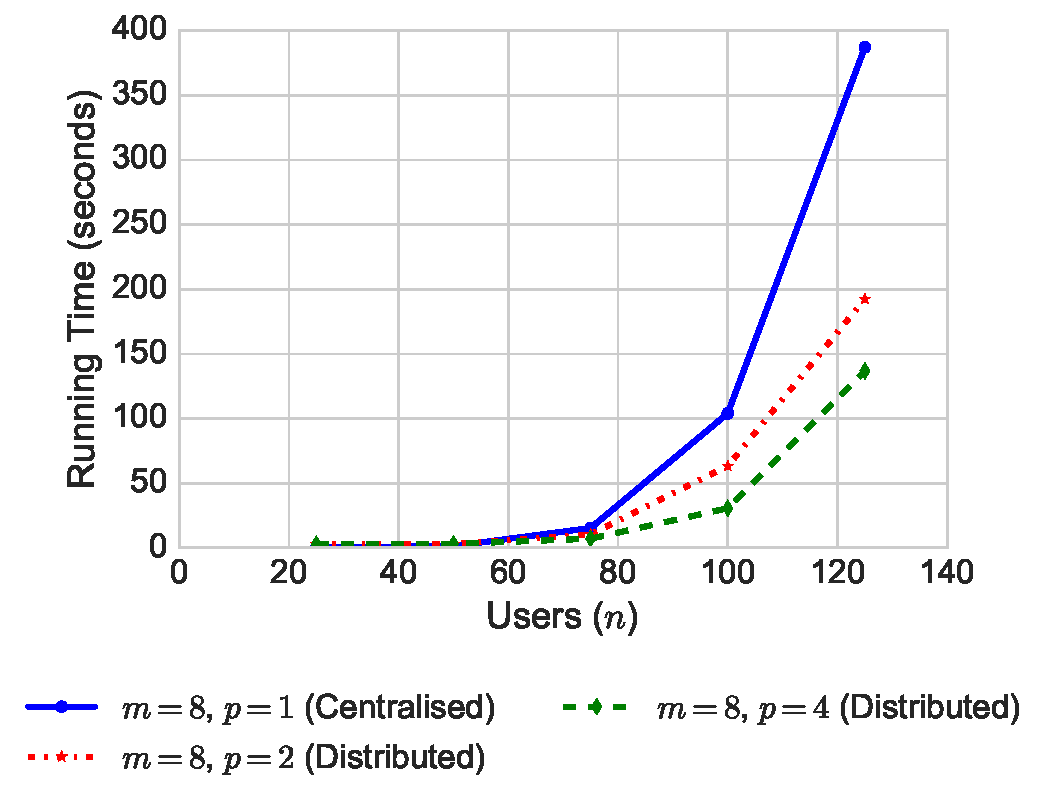
\includegraphics[width=0.65\columnwidth,keepaspectratio]{time-vcg}
	\caption{Running time for standard auction}
	\label{fig:standard-auction-time}
\end{figure}
 

% *** Section: Related Work
%
%
%% Section: RELATED WORK
%\section{Related Work}
%\label{sec:related-work}
%
%The idea of collaboratively built community clouds follows on from earlier distributed voluntary computing platforms, like 
%	BOINC~\cite{Anderson2004},
%	Folding@home~\cite{Beberg2009}, 
%	HTCondor~\cite{Thain2005}, 
%	PlanetLab~\cite{Chun2003}
%	and Seattle~\cite{Cappos2009}, 
%which mainly rely on altruistic contribution of resources from the users, 
%though various mechanisms have been studied in the context of peer-to-peer systems~\cite{Shen2010} 
%that address different problems of collaborative resource sharing. 
%There are only a few research proposals for community cloud computing~\cite{Marinos2009}. 
%Most of them do not go beyond the level of an architecture, and at most a practical implementation is presented.
%None of these implementations, to our knowledge, are actually being deployed inside of real community networks. 
%
%The Cloud@Home\cite{Distefano2012} project aims to harvest in resources from the community for meeting the peaks in demand, working with public, private and hybrid clouds to form cloud federations.
%The authors propose a rewards and credit system for ensuring quality of service.
%Gall et al.~\cite{Gall2013} have explored how an InterCloud architecture~\cite{Buyya2010InterCloud} can be adapted to community clouds.
%Social cloud computing~\cite{Chard2012} takes advantage of the trust relationships between members of social networks to motivate contribution towards a cloud storage service. 
%Users trade their excess capacity to earn virtual currency and credits that they can utilize later, and consumers submit feedback about the providers after each transaction which is used to maintain reputation of each user.
%Social clouds have also been deployed in CometCloud framework by federating resources from multiple cloud providers~\cite{Punceva2013}.
%Zhao et al.~\cite{Zhao2014} explore efficient and fair resource sharing among the participants in community-based cloud systems.
%Jang et al.\cite{Jang2014} implement personal clouds that combine local, nearby and remote cloud resources to enhance the services available on mobile devices.
%
%From the review of related work, we find that none of the above cases correspond to the concrete situation of community networks such as targeted by us. 
%In the cloud system that we propose, we aim to take into account several of the important factors that characterize community networks, such as the scenarios we identified from the conditions of community networks.


% *** Section: Future Work
%
%
%\section{Discussion}
%\label{sec__discussion}

% *** Section: Conclusion


Cloud computing with its success in providing virtualised resources on demand has transformed the technology landscape, revolutionising how Internet applications are developed and delivered to the users.
Peer-to-peer and edge computing models have been explored in the past decade, but other than a few success stories they never made it big in the mainstream.
Perhaps now is the right opportunity to take full advantage of the virtualization model of the cloud computing to design the killer applications for the community cloud.
On the technical side, this allows for sophisticated applications and services that were not possible with the simple process-level isolation approaches of earlier efforts like BOINC or Seattle.
The challenge is to provide developer tools and middleware services that streamline the process of programming and deploying the community cloud applications.
At the same time, killer applications are needed that by satisfying users' critical needs and problem scenarios succeed in engaging the community for the long-term.

In this thesis, we looked at the field of community clouds in general, 
and clouds in community networks in particular,
to develop economic regulation mechanisms in tune with 
the specific social, economic and technical context of the community networks
in order to help us in developing and sustaining a community cloud ecosystem.
We looked at how these mechanisms fit in an overall framework of a community cloud system,
which supports components for 
	incentivising contribution, 
	regulating access to resources, 
	and ensuring trust in the system.
We developed incentive-based resource regulations mechanisms for a well-knit community of trusted users,
and showed how they are crucial for successful operation of a community cloud.
We also noticed how lack of trust in a community cloud deployed on a large scale affects negatively the utility and sustainability of the system.
To address this issue, we developed a distributed auctioneer component, 
which is a virtual trusted entity integrated in the overall architecture of the community cloud.
This component allows to efficiently and optimally allocate resources in a community of untrusted users,
with negligible communication and computation overhead, 
and it can also leverage parallelised implementation to offer scalability.


% use section* for acknowledgement
\section*{Acknowledgement}
This work was supported by the European Community Framework Programme~7 FIRE Initiative projects Community Networks Testbed for the Future Internet (CONFINE), FP7-288535, and CLOMMUNITY, FP7-317879. 
Support is also provided by the Universitat Polit\`ecnica de Catalunya BarcelonaTECH and the Spanish Government through the Delfin project TIN2010-20140-C03-01.


%
% ---- Bibliography ----
%
\bibliographystyle{LNCSTemplate/splncs}
\bibliography{Bibliography/references}
%


%\clearpage
%\addtocmark[2]{Author Index} % additional numbered TOC entry
%\renewcommand{\indexname}{Author Index}
%\printindex
%\clearpage
%\addtocmark[2]{Subject Index} % additional numbered TOC entry
%\markboth{Subject Index}{Subject Index}
%\renewcommand{\indexname}{Subject Index}
%\input{subjidx.ind}

\end{document}
